\documentclass[conference]{IEEEtran}
\usepackage{graphicx}
\usepackage{amsfonts}
\usepackage[hyphens]{url}

\ifCLASSINFOpdf
\else
\fi

\begin{document}

\title{CSCI 447 Project 2: Neural Networks \\ Fall 2015}

\author{
  \IEEEauthorblockN{Brandon Fenton}
  \IEEEauthorblockA{Department of Mathematical Sciences\\
    Montana State University\\
    Bozeman, MT 59717\\
    Email: brandon.fenton@gmail.com}
  \and
  \IEEEauthorblockN{Jenna Lipscomb}
  \IEEEauthorblockA{Department of Computer Science\\
    Montana State University\\
    Bozeman, MT 59717\\
    Email: jennalynnlipscomb@gmail.com}
  \and
  \IEEEauthorblockN{John Sherrill}
  \IEEEauthorblockA{Department of Mathematical Sciences\\
    Montana State University\\
    Bozeman, MT 59717-2400\\
    Email: prof.sherrill@gmail.com}}

\maketitle

\begin{abstract}
  Two machine learning frameworks, a radial basis function network and a feedforward neural network, were created to approximate the generalized Rosenbrock function for a variable number of dimensions. An iterative k-fold cross validation process was implemented for both networks to tune model parameters and the resultant models were tested on a final large-scale test set to evaluate performance and thus compare the two different frameworks in the context of function approximation for this particular example. It was hypothesized that the feedforward neural network would possibly be able to model the algebraic representation of the Rosenbrock function and would thus outperform the radial basis function network. \textit{This hypothesis was refuted by sound evidence from the model evaluation process indicating the the radial basis function performs better in this context}. The radial basis function network was trained by a recursive least squares implementation that was hypothesized to be significantly faster than the backpropogation algorithm used in training the feedforward neural network. \textit{This was confirmed in all of the different configurations for testing the networks}. 
  
\end{abstract}

\section{Introduction}
\label{intro}
The generalized $N$-dimensional Rosenbrock function may be expressed as

$$
f(\mathbf{x}) = \sum_{i=1}^{N-1} 100 (x_{i+1} - x_i^2 )^2 + (1-x_i)^2
$$$$
  \mbox{where} \quad \mathbf{x} = [x_1, \ldots, x_N] \in \mathbb{R}^N.
$$

This function was approximated for $N$ = 2, 3, 4, 5, and 6 with each dimension constrained on the interval -1.5 to 1.5. That is, the domain was a 2, 3, 4, 5, and 6 dimensional hypercube $ \mathbf{x} \in [-1.5, 1.5]^N$, $N \in \{2,3,4,5,6\}$.

These functions were to be approximated using a feedforward neural network and radial basis function network. The broad goal of this exercise was two fold: 1) comparing the rate of convergence to an exceptable level of error between the two frameworks and 2) comparing final model performance.
  
\section{Network and Algorithm Descriptions}
Two neural networks with different training algorithms were implemented. A feedforward neural (FFN) network framework was created that utilizes stochastic gradient descent via the now famous backpropogation algorithm \cite{rumelhart}. A radial basis function (RBF) network framework was also created that utilizes a $k$-means clustering algorithm for initializing model parameters (to be described in more detail below) and recursive least squares method for iteratively updating the model.

  \subsection{Feedforward Neural Network}
  A standard FFN network consists of a sequence of $l$ layers, each consisting of $n_i$ different ``nodes''. The first layer is called the input layer and unsurprising takes as input the $d_{in}$ different attributes of the data to be modeled. Thus, $n_1 = d_{in}$. The last layer is called the output layer and also unsurprising provides the output of the network, i.e. the predicted value for the attribute to be predicted. Thus, if the dimensionality of the output space is $d_{out}$, then $n_l = d_{out}$. The other $l-2$ layers inbetween the input and output layers are referred to as hidden layers. Each node in hidden layer $i$ is connected with all nodes in layer $i-1$ and $i+1$. Lastly, the edges in the graph described are all unidirectional, such that if one begins at an input node, one nescissarily ends at an output done. A simple 3 layer network is presented visually in Fig. \ref{fig:exampleNetwork} where $n_1 = 4$, $n_2 = 5$, and $n_3 = 1$.

  \begin{figure}
    \centering
    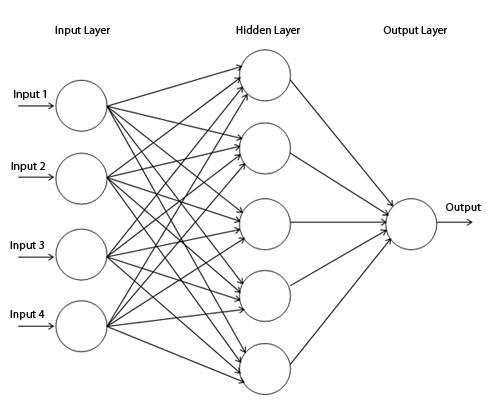
\includegraphics[width=\linewidth]{network.jpg}
    \caption{Example Neural Network}
    \label{fig:exampleNetwork}
  \end{figure}

  Excluding the edges contected to the input layer, for each edge there is an associated weight. Nodes take as input the weighted sum of outputs from their upsteam nodes plus a bias term specific to each node (a node in layer $i$ is considered upstream from nodes in layers $j>i$ and a node in layer $i$ is considered downstream from nodes in layers $j<i$). In the implementation provided, weights and biases are initialized to random values. The output value of a node is the value of a network-wide specified activation function of the input to the node. A typical activation function used is the logistic function or the hyperbolic tangent function. For this project, both the logistic function and a linear activation function were implemented with the choice left up to the user. If the linear activation function is chosen a slope must be supplied.

    \subsubsection{Training}
    Training for FFN networks is generally accomplished by a task often referred to as ``backpropogation''. In general terms, the error between predicted output and target output is propogated back through the network to provide information to be able to perform a gradient descent through the parameter space (the space of all possible weights and bias values).
  
  \subsection{Radial Basis Function Network}
  An RBF network has the same topology as a FFN network except there is only one hidden layer. RBF networks are also unidirection. The graphic in Fig. \ref{fig:exampleNetwork} also represents an RBF network topoloy.

  The defining difference between the two networks is that RBF networks use \textit{radial basis functions} for activation functions. A radial basis function, $\phi(\mathbf{x}, \mathbf{c})$, is a function solely of the distance between points $\mathbf{x}$ and $\mathbf{c}$: $||\mathbf{x} - \mathbf{c}||$. A typical choice for the basis function (and the one chosen for the provided implementation) is a Gaussian basis function:
  $$
  \phi(\mathbf{x}) = e^{-\beta ||\mathbf{x} - \mathbf{c}||^2}
  $$
  where $\beta$ is a user-specified, tunable parameter.
  For each node $i$ in the hidden layer (referred to as ``Gaussian Nodes'' or simply ``Gaussians'') the centers of the basis function, $\mathbf{c}_i$ are different.

  The only edges in the network that have associated weights $w_i$ are the edges connecting the hidden layer to the output layer. While not necessary, a bias term $b$ is included in the authors implementation. Thus, the predicted output $o$, given input $\mathbf{x}$, of an RBF network with $k$ Gaussians and one dimensional output is
  $$
  o = \sum_{i=1}^k w_i e^{-\beta ||\mathbf{x} - \mathbf{c_i}||^2} + b.
  $$
  
    \subsubsection{Training}
    The training process for RBF networks is customarily divided into two parts. The first step is choosing appropriate centers for the radial basis functions of the Gaussian nodes. Often this is performed by using the $k$-means clustering algorithm. Such an algorithm is used by the authors for this step.

    Once the Gaussian centers have been chosen, the model weights and bias may be learned. This may be accomplished by a variety of methods. The two most common being gradient descent and ordinary least-squares minimization. Given a training data set $D = \{\mathbf{x}_j\}_{j=}^N$, there is a closed form expression given by a generalized inverse of an appropriately organized matrix of the training data. Computation of matrix inverses is, however, computationally laborious and is not well suited for very large RBF networks.

    Recursive least squares provides a more efficient method that allows for continual learning and updating of the weights and bias. Given one training point, an update to the weights and bias can be expressed in terms of scalar and matrix multiplication (technically a matrix inverse is computed but is an inverse of a 1 by 1 matrix (division)). Thus, the only step at which a matrix inverse is required to compute is at the initialization step when starting values of weights and bias are chosen. While it is possible to randomly assign weights, this would be providing irremovable error into parameter estimation that would be impossible to remove. The method the authors chose was as follows: given an RBF network with $k$ Gaussians, compute the least-squares minimizing weights and bias for $k$ training points (using the generalized inverse). Then iteratively update the weights and bias by recursive least squares.
    
\section{Experimental Approach}
  \subsection{Tuning}
  Searching a grid for all possible tuning parameters proved to be impractical given the slow speed of the learning process of the various algorithms. A less intensive approach was taken that randomly sampled from the tuning parameter space \cite{bergstra}.
  
  \subsection{$k$-fold Cross-Validation}

\section{Results}
  \subsection{Model Performance}

  \subsection{Convergence}
  
\begin{table}[H]
  \caption{Relation Sizes}
  \resizebox{1.3\textwidth}{!} {\begin{minipage}{\textwidth}

      \begin{tabular}{ | c | c |}
        \hline
        Relation Name & number of entities $(n)$ \\ \hline
        \texttt{CHAMPIONS} & 122 \\
        \texttt{ITEMS} & 280 \\
        \texttt{BANNED} & 19,874 \\
        \texttt{MATCH-CHAMPS} & 9,892 \\
        \texttt{MATCH-CHAMP-ITEMS} & 62,781 \\
        \texttt{MATCH-CHAMP-STREAKS} & 4,478 \\ \hline
      \end{tabular}

      \label{table:sizeTable}
  \end{minipage} }
\end{table}

\section{Conclusion}


\begin{thebibliography}{1}

\bibitem{rumelhart}
  Rumelhart, D. E., Hinton, G. E., and Williams, R. J. (1986). Learning internal representations by error propagation. Parallel Distributed Processing: Explorations in the Microstructure of Cognition. Volume 1: Foundations Volume 1: Foundations, MIT Press, Cambridge, MA.

\bibitem{bergstra}
  Bergstra, J., Bengio, Y. (2012). Random Search for Hyper-Parameter Optimization. Journal of Machine Learning Research. Volume 13. 281 - 305.

\bibitem{fenton}
  Fenton, B., Sherrill, J. (2015). Github repository containing code: https://github.com/joncheryl/csci447/tree/master/project2.

\end{thebibliography}

\end{document}
